\chapter{Evaluation and Testing}
\section{Introduction}
This section will review the work undertaken in chapter 3: Design and Implementation. Chapter 3 broke the workflow down to 5 main headings, here 3 headings are discussed in relation to the outcome of the processes.

\section{Results of Clustering}
In section 3.2.3: Clustering Time Series Data, hierarchical clustering was performed. Here the maxcluster parameter in the fclusters() function was chosen to be 3. Why was 3 chosen? As it's unknown the true number clusters contained in the data set and as we're clustering on average consumption as the metric, it is assumed that the data set will be partitioned into low, medium and high energy consumers. The results of the hierarchical clustering can be shown in the form of the dendrogram below in fig 4.1. It shows the index of each ANON\_ID on the x-axis, and the distance metric on the y-axis. This graph shows how ANON\_IDs are paired with the most similar and how pairs then make up the new combined series. All ANON\_IDs were assigned a cluster ID to which will be used later for classification using a Random Forest model.
\begin{figure}
\centering     
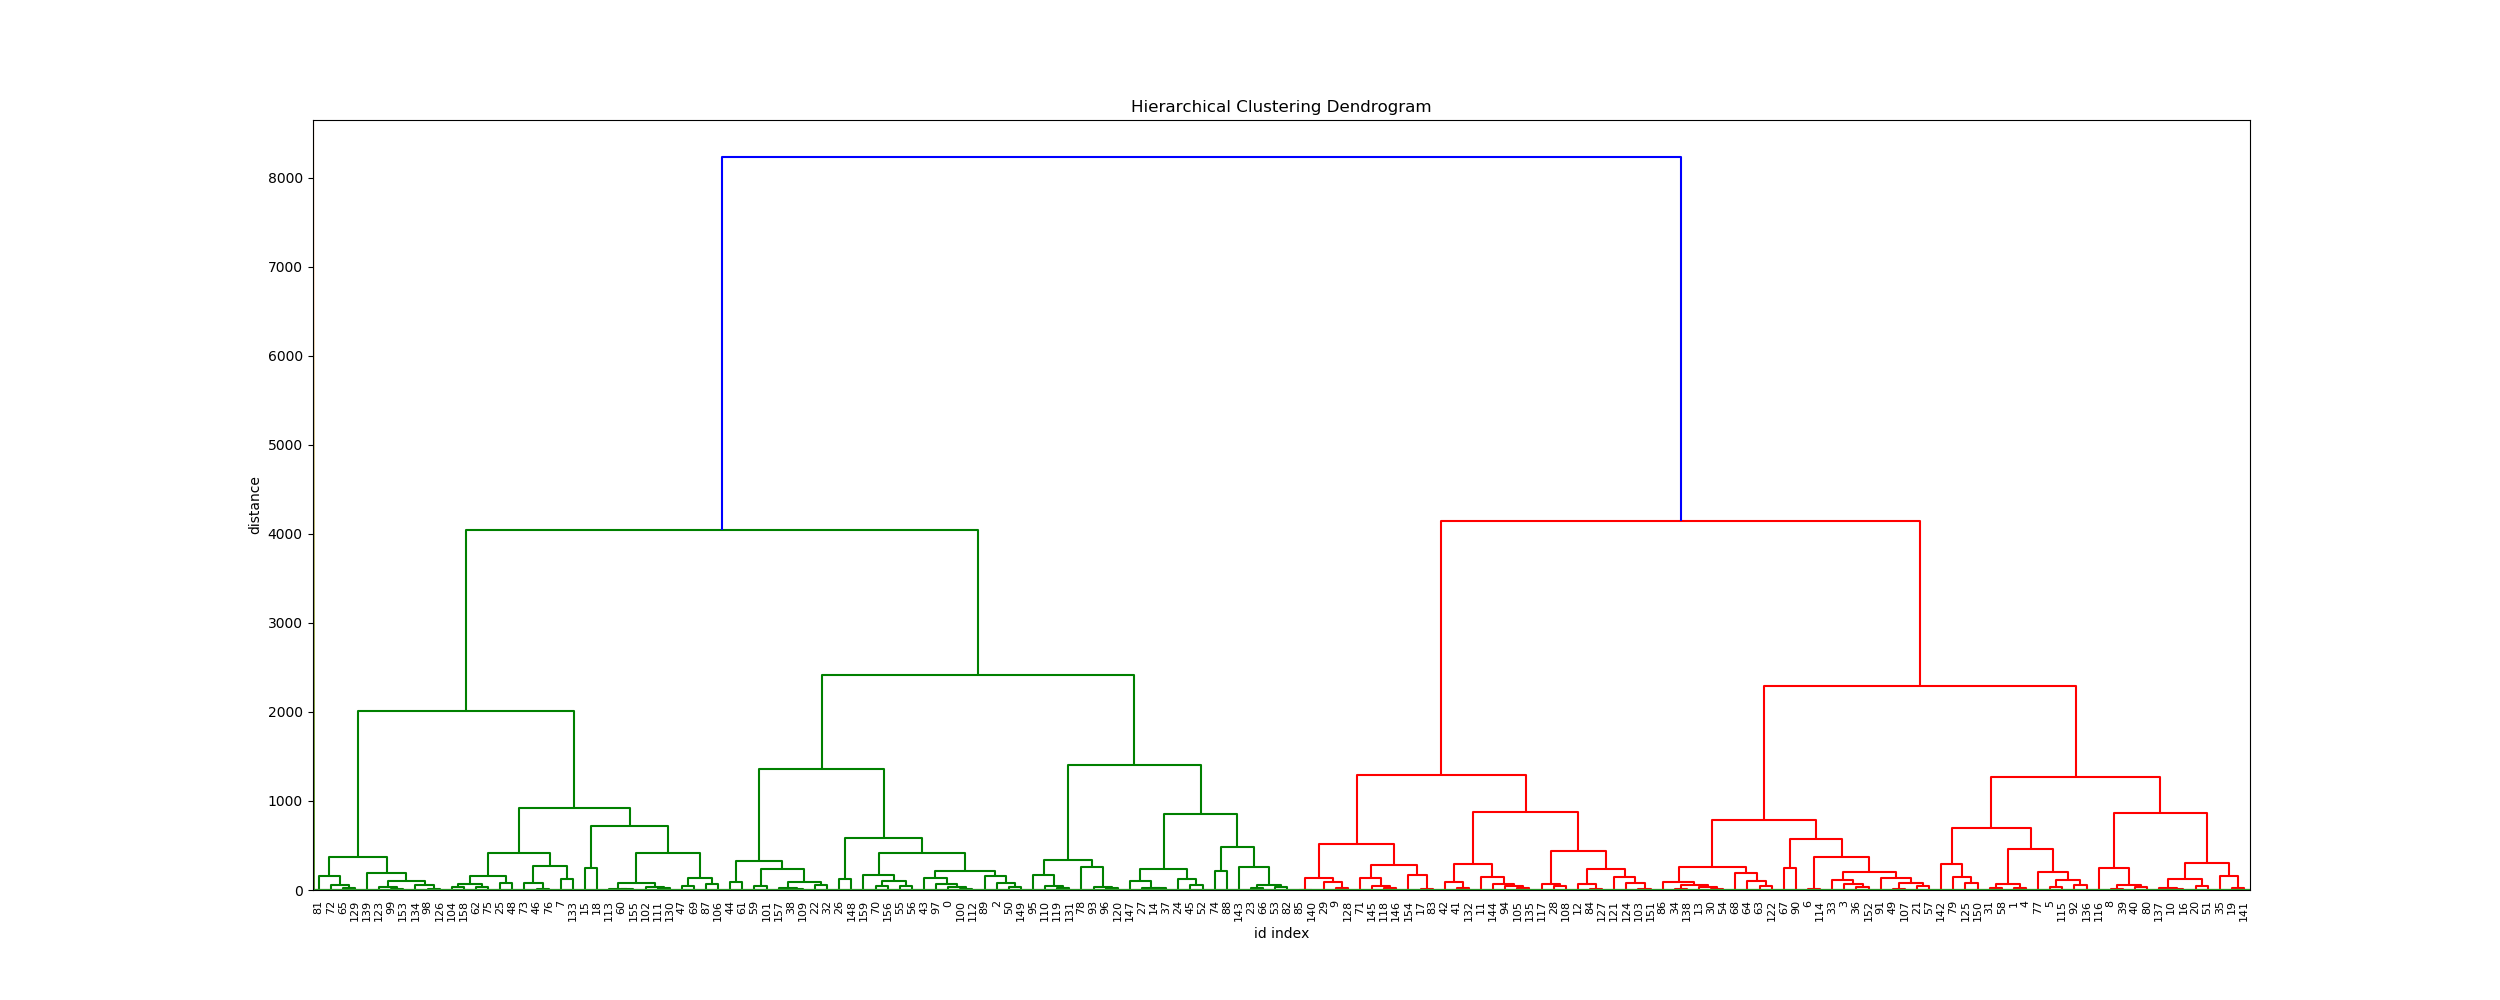
\includegraphics[width=1.5\textwidth, angle=90]{Figures/clusters_time_series.png}
\caption{Dendogram Generated from results of Hierarchical Clustering}
\label{fig:Dendrogram}
\end{figure} 

\subsection{Analysis of Clustering Results}
By assigning each ANON\_ID to a cluster then merging the time series consumption data along with the Geographies data set, data analysis can now be performed on the results of the clustering.

\begin{itemize}
    \item cluster frequency
    \item mean, min, max energy consumption per cluster
    \item correlation matrix, cluster with survey data
    \item further graphs with clusters \& survey data
\end{itemize}


\section{Results of Random Forest Model}
In this section, the performance of the random forest model built will be evaluated with reference various graphs generated.